\documentclass[a4,13pt]{extarticle}
\usepackage[utf8]{inputenc}
\usepackage[margin=2cm]{geometry}
\usepackage{amsmath}
\usepackage{graphicx}
\usepackage{algorithm}
\usepackage{algorithmicx}
\usepackage[]{algpseudocode}
\usepackage{hyperref}
\usepackage{color}

\definecolor{blue}{rgb}{0,0,0.5}
\newenvironment{Solution}{\color{blue}\textbf{Solution:}}{}

\title{COMP3506 Homework 1}
\author{Weighting: 15\%}
\date{Due date: 21st August 2020, 11:55 pm}

\begin{document}

\maketitle

\section*{Questions}

\begin{enumerate}
	\item   
	      Consider the following algorithm, \textsc{CoolAlgorithm}, which takes a \textbf{positive} integer $n$ and outputs another integer. 
	      Recall that `$\&$' indicates the bitwise AND operation and `$a >> b$' indicates the binary representation of $a$ shifted to the right $b$ times.
	      	      
	      \begin{algorithm}
	      	\begin{algorithmic}[1]
	      		\Procedure{CoolAlgorithm}{int n}
	      		\State $sum \gets 0$
	      		\If {$n$ \% $2 == 0$}
	      		\For{$i=0$ to $n$} 
	      		\For {$j=i$ to $n^2$}
	      		\State $sum \gets sum + i + j$ 
	      		\EndFor 
	      		\EndFor
	      		\Else
	      		\While{$n > 0$}
	      		\State $sum \gets sum$ + $(n$ \& $1)$
	      		\State $n \gets (n >> 1)$
	      		\EndWhile
	      		\EndIf
	      		\State \textbf{return} $sum$
	      		\EndProcedure
	      	\end{algorithmic}
	      \end{algorithm}
	      	          
	      Note that the runtime of the above algorithm depends not only on the size of the input $n$, but also on a numerical property of $n$. 
	      For all of the following questions, you must assume that $n$ is a positive integer.
	      	      
	      \begin{enumerate}
	      	\item (3 marks) Represent the running time (i.e. the number of primitive operations) of the algorithm when the input $n$ is \textbf{odd}, as a mathematical function called $T_{\text{odd}}(n)$. State all assumptions made and explain all your reasoning.
	      	      
			\begin{Solution}

				In the above pseudocode for an odd $n$, a while loop is run for $n$ iterations. Within the loop 3 primitive operations (a bitwise AND, an addition and a single bitshit) are all performed. This means that each of the 3 primitive operations are run $n$ and hence $T_{odd}(n) = 3n$ for both the tight and worse-case bounds.
			\end{Solution}

			\medskip
	      	      	      	                  
	      	\item (2 marks) Find a function $g(n)$ such that $T_{\text{odd}}(n)\in O(g(n))$. Your $g(n)$ should be such that the Big-O bound is as tight as possible (e.g. no constants or lower order terms). Using the formal definition of Big-O, prove this bound and explain all your reasoning. 
	      	      	      	                  
	      	(Hint: you need to find values of $c$ and $n_0$ to prove the Big-O bound you gave is valid).
	      	      
			\begin{Solution}

				Using the definition of Big-O: $f(n)$ is $O(g(n))$ if there exists a real number $c > 0$ and real number $n_0 > 0$ such that $f(n) \leq cg(n)$, for $n \geq n_0$.

				The constants $c = 3$ and $n_0 = 1$ can be substituted to show that $T_{odd}(n) = 3n$ is $O(n)$ and thus $g(n) = n$. $f(n) = 3n$ and $cg(n) = 3n$ as well, so for all $n \geq 1$, $f(n)$ and $cg(n)$ must all be equal. This satisfies the conditions of the Big-O definition and hence it is proven that $g(n) = n$.
			\end{Solution}

			\medskip
	      	      	      	                  
	      	\item (2 marks) Similarly, find the tightest Big-$\Omega$ bound of $T_{\text{odd}}(n)$ and use the formal definition of Big-$\Omega$ to prove the bound is correct. Does a Big-$\Theta$ bound for $T_{\text{odd}}(n)$ exist? If so, give it. If not, explain why it doesn't exist.
	      	
			\begin{Solution}

				Using the definition of Big-$\Omega$: $f(n)$ is $\Omega(g(n))$ if there exist positive constants $c$ and $n_0$ such that $f(n) \geq cg(n)$ for all $n \geq n_0$.

				Once again, the constants $c = 3$ and $n_0 = 1$ can be substituted to show that $T_{odd}(n) = 3n$ is $\Omega(n)$ and thus $g(n) = n$. Taking, $f(n) = 3n$ and $cg(n) = 3n$, it is clear that for all $n \geq 1$, $f(n) = cg(n)$ and hence the definition is satisfied.
				
				\medskip

				A Big-$\Theta$ bound does exist. Using the definition of Big-$\Theta$: $f(n)$ is $\Theta(g(n))$ if there exist positive constants $c_1$, $c_2$ and $n_0$ such that $c_1g(n) \leq f(n) \leq c_2g(n)$ for all $n \geq n_0$.

				Since the Big-O and Big-$\Theta$ bounds are both $n$, the constants $c_1 = c_2 = 3$ and $n_0 = 1$ can be used. This would result in $c_1g(n) = c_2g(n) = 3n$ which is also equal to $f(n)$ for all $n \geq 1$. Thus the above definition is satisfied and the Big-$\Theta$ bound must be $\Theta(n)$. 
	      	\end{Solution}
								  
			\medskip
	      	      	      	                  
	      	\item (3 marks) Represent the running time (as you did in part (a)) for the algorithm when the input $n$ is \textbf{even}, as a function called $T_{\text{even}}(n)$. State all assumptions made and explain all your reasoning. Also give a tight Big-O and Big-$\Omega$ bound on $T_{\text{even}}(n)$. You do \textbf{not} need to formally prove these bounds.
	      	
			\begin{Solution}
			
				If $n$ is even, there is a loop that loops $n$ times with a nested loop that operates $n^2$ times. Within the nested loop there are two add operations and hence two primitive operations. Thus the running time $T_{\text{even}}(n) = n \times n^2 \times 2 = 2n^3$.

				\medskip

				The Big-O bound must thus be $O(n^3)$ and the Big-$\Theta$ is also $\Theta(n^3)$. These are both the tightest bounds.
			\end{Solution}
			\medskip
	      	      	      	                  
	      	\item (2 marks) The running time for the algorithm has a best case and worst case, and which case occurs for a given input $n$ to the algorithm depends on the parity of $n$.
	      	      	      	                  
			Give a Big-O bound on the \textbf{best case} running time of the algorithm, and a Big-$\Omega$ bound on the \textbf{worst case} running time of the algorithm (and state which parity of the input corresponds with which case).

			\begin{Solution}
				
				The best case running time of the algorithm occurs when the input $n$ is odd. This is because the running time for odd $n$ is $3n$ whereas the running time for even $n$ is $2n^3$. The Big-O bound for the odd case is $O(n)$.

				Conversely, the worst case must be for the even case or when the running time is $2n^3$. The Big-$\Omega$ for this case is $O(n^3)$.

				Both of these bounds have been proven in previous sections.
			\end{Solution}
			  
			\medskip     	      	      	      
	      	      	      	                  
	      	\item (2 marks) We can represent the runtime of the entire algorithm, say $T(n)$, as
	      	      \begin{align*}
	      	      	T(n)=\begin{cases}
	      	      	T_{\text{even}}(n) & \text{if $n$ is even} \\
	      	      	T_{\text{odd}}(n)  & \text{if $n$ is odd}  \\
	      	      	\end{cases}
	      	      \end{align*}
	      	      Give a Big-$\Omega$ and Big-$O$ bound on $T(n)$ using your previous results. If a Big-$\Theta$ bound for the entire algorithm exists, describe it. If not, explain why it doesn’t exist.
	      	      
			\begin{Solution}
				The Big-O bound for $T(n)$ is $O(n^3)$ and the Big-$\Omega$ bound for $T(n)$ is $\Omega(n)$. This is because only $n^3$ is the tightest bound that is greater than or equal to $T(n)$ for any $n > 1$ and $n$ is the tightest bound that is less than or equal to $T(n)$ for any $n > 1$.

				\medskip

				There is no Big-$\Theta$ bound for this algorithm as there is no $g(n)$ that could be less than $T(n)$ when multiplied by one constant while being greater than $T(n)$ when multiplied by another constant. This is because $T_{\text{even}}(n)$ is a third degree polynomial and $T_{\text{odd}}(n)$ is a linear function. Thus any $g(n)$ would cross through either of subfunctions of $T(n)$. So, the requisites of Big-$\Theta$ bound are not met and so there is no Big-$\Theta$ bound.
	      	\end{Solution}
						   
			\medskip

	      	\item (2 marks) Your classmate tells you that Big-O represents the worst case runtime of an algorithm, and similarly that Big-$\Omega$ represents the best case runtime. Is your classmate correct? Explain why/why not. Your answers for (e) and (f) \textit{may} be useful for answering this.
	      	      
			\begin{Solution}
				Tight Big-O and Big-$\Omega$ represent the worst case time complexity and best case time complexity, respectively. This is not exactly the same as runtime and instead simply provides a class for the algorithm. The runtime could be better or worse than the Big-O and Big-$\Omega$ time complexity due to constants and other factors.
				
				Furthermore, while a tight Big-O and Big-$\Omega$ bound can represent the worst case and best case respectively, it is possible for non-tight bounds to exist. For example, all algorithms can be said to be $\Omega(1)$, however that does not mean they ever actually run with that time complexity. 
			\end{Solution}
			  
			\medskip
	      	      	      	                  
	      	\item (1 mark) Prove that an algorithm runs in $\Theta (g(n))$ time if and only if its worst-case running time is $O(g(n))$ and its best-case running time is $\Omega(g(n))$.
	      	      
			\begin{Solution}
				By definition an algorithm with running time $f(n)$ is $O(g(n))$ if there exist some positive constants $c$ and $n_0$ such that $f(n) \leq cg(n)$ for all $n \geq n_0$. As such, Big-O defines the worst case time complexity for sufficiently large inputs.
				
				$f(n)$ is also $\Omega(g(n))$ if there exist some positive constants $c$ and $n_0$ such that $f(n) \geq cg(n)$ for all $n \geq n_0$. As such, Big-$\Omega$ defines the best case time complexity for sufficiently large inputs.

				$f(n)$ is also $\Theta(g(n))$ if there exist some positive constants $c_1$, $c_2$ and $n_0$ such that $c_1g(n) \leq f(n)\leq c_2g(n)$ for all $n \geq n_0$.

				Taking an algorithm that is $\Theta(g(n))$, there must be some $c_1$, $c_2$ and $n_0$ such that $c_1g(n) \leq f(n) \leq c_2g(n)$ for all $n \geq n_0$. Hence, by definition the algorithm is also $O(g(n))$ and $\Omega(g(n))$ as $f(n) \leq c_2g(n)$ fulfills the definition of Big-O and $c_1g(n) \leq f(n)$ fulfills the definition of Big-$\Omega$. Hence the algorithm is both $O(g(n))$ and $\Omega(g(n))$ given it is $\Theta(g(n))$.

				Similarly taking the other end of the argument, that is an algorithm that is both $O(g(n))$ and $\Omega(g(n))$. Meaning that there exists some $c_1$, $n_0$ such that $f(n) \leq c_1g(n)$ for all $n \geq n_0$ and there exists some $c_2$, $n_0$ such that $f(n) \geq c_2g(n)$ for all $n \geq n_0$. Combining these statements into a single inequality gives $c_2g(n) \leq f(n) \leq c_1g(n)$ for all $n \geq n_0$ meaning that the definition of Big-$\Theta$ is fulfilled and the algorithm is $\Theta(g(n))$.

				Since, it has been proven that if an algorithm runs in $\Theta(g(n))$ it must run in $O(g(n))$ and $\Omega(g(n))$ and it has also been proven that if an algorithm runs in $O(g(n))$ and $\Omega(g(n))$ it must run in $\Theta(g(n))$ the implication has been proven. That is, it has been proven that an algorithm is $\Theta(g(n))$ if and only if it is $O(g(n))$ and also $\Omega(g(n))$.
	      	\end{Solution}
	      	      	      	                  
	      \end{enumerate}
	      	          
	      \newpage 
	      	
	\item 
	      \begin{enumerate}
	      	\item (4 marks) Devise a \textbf{recursive} algorithm that takes a sorted array $A$ of length $n$, containing distinct (not necessarily positive) integers, and determines whether or not there is a position $i$ (where $0\leq i < n$) such that $A[i] = i$.
	      	      \begin{itemize}
	      	      	\item Write your algorithm in pseudocode (as a procedure called $\textsc{FindPosition}$ that takes an input array $A$ and returns a boolean).
	      	      	\item Your algorithm should be as efficient as possible (in terms of time complexity) for full marks.
	      	      	\item You will not receive any marks for an iterative solution for this question. 
	      	      	\item You are permitted (and even encouraged) to write helper functions in your solution.
	      	      \end{itemize}
	      	      
			\begin{Solution}

				\begin{algorithm}
					\begin{algorithmic}[1]
						\Procedure{FindPosition}{int[] A}
						\State \textbf{return} FindPositionHelper(A, 0, length(A))
						\EndProcedure
					\end{algorithmic}
				\end{algorithm}
				\medskip
				\begin{algorithm}
					\begin{algorithmic}[1]
						\Procedure{FindPositionHelper}{int[] A, int n, int length}
						\State $middle \gets n + length/2$
						\If {$A[middle] = middle$}
							\State \textbf{return} true
						\EndIf
						\\
						\If {$length = 1$}
							\State \textbf{return} false
						\EndIf
						\\
						\If {$A[middle] > middle$}
							\State \textbf{return} FindPositionHelper(A, 0, length/2)
						\EndIf
						\\
						\If {$A[middle] < middle$}
							\State \textbf{return} FindPositionHelper(A, length/2, length/2)
						\EndIf
						\EndProcedure
					\end{algorithmic}
				\end{algorithm}
				\medskip
	      	\end{Solution}
	      	
	      	\item (1 mark) Show and explain all the steps taken by your algorithm (e.g. show all the recursive calls, if conditions, etc) for the following input array: $[-1,0,2,3,10,11,23,24,102]$.
	      	
			\begin{Solution}

				FindPosition($[-1, 0, 2, 3, 10, 11, 23, 24, 102]$) \\
				\null\qquad \textbf{return} FindPositionHelper($[-1, 0, 2, 3, 10, 11, 23, 24, 102]$, $0$, $9$) \\
				FindPositionHelper($[-1, 0, 2, 3, 10, 11, 23, 24, 102]$, $0$, $9$) \\
				\null\qquad middle $= 0 + \frac{9}{2} = 4$ \\
				\null\qquad if $A[4] = 4 \rightarrow$ false \\
				\null\qquad if length $= 1 \rightarrow$ false \\
				\null\qquad if $A[4] > 4 \rightarrow$ true \\
				\null\qquad\qquad \textbf{return} FindPositionHelper($[-1, 0, 2, 3, 10, 11, 23, 24, 102]$, $0$, $4$)

				FindPositionHelper($[-1, 0, 2, 3, 10, 11, 23, 24, 102]$, $0$, $4$) \\
				\null\qquad middle $= 0 + \frac{4}{2} = 2$ \\
				\null\qquad if $A[2] = 2 \rightarrow$ true \\
				\null\qquad\qquad \textbf{return} true

	      	\end{Solution}
	      	      	      	                  
	      	\item (3 marks) Express the worst-case running time of your algorithm as a mathematical recurrence, $T(n)$, and explain your reasoning. Then calculate a Big-O (or Big-$\Theta$) bound for this recurrence and show all working used to find this bound (Note: using the Master Theorem below for this question will not give you any marks for this question).
	      	      
	      	      
			\begin{Solution}
				The worst case scenario occurs when there is no value where $A[i] = i$ and all $A[i] < i$. In this scenario, there are 11 primitive operations inside each of the function calls as the final if statement is the only one evaluated to true each time. Each time the function is recursively called, however, the length of the array is halved. The final call of the helper function (where $n = 1$) takes 7 primitive operations as it reaches the false base case. As such the recurrence for the running time can be presented as:

				\begin{align*}
					T(n) = \begin{cases}
						T(\frac{n}{2}) + 11 & \text{if } n > 1
						\\
						7 & \text{if } n = 1
					\end{cases}
				\end{align*}

				Where $n$ is the length of the array inputted into FindPosition. 

				Taking the case where $n > 1$:
				
				\begin{align*}
					T(n) & = T(\frac{n}{2}) + 11 \\
						 & = T(\frac{n}{4}) + 22 \\
						 & = T(\frac{n}{8}) + 33 \\
						 & = T(\frac{n}{16}) + 44 \\
						 & = T(\frac{n}{2^k}) + k \times 11 \\
				\end{align*}

				In order to reach the $T(1)$ case of the recurrence relation, $k$ can be taken as $k = log(n)$ and substituted into $T(n)$:

				\begin{align*}
					T(n) & = T(\frac{n}{2^k}) + 11log(n) \\
						 & = T(\frac{n}{2^{log(n)}}) + 11log(n) \\
						 & = T(\frac{n}{n}) + 11log(n) \\
						 & = T(1) + 11log(n) \\
						 & = 7 + 11log(n) \\
				\end{align*}

				Therefore, $T(n)$ is $O(log(n))$ in the worst case. This can be proven by taking $c = 18$ and $n_0 = 2$ resulting in $T(n) \leq 18 log(n)$ for all $n \geq 2$ which satisfies the definition of Big-O.
	      	\end{Solution}
	      	
	      	\item The master theorem is a powerful theorem that can be used to quickly calculate a tight asymptotic bound on a mathematical recurrence. A simplified version is stated as follows: Let $T(n)$ be a non-negative function that satisfies
	      	      \begin{align*}
	      	      	T(n)                              & = \begin{cases}    
	      	      	aT\left(\frac{n}{b}\right) + g(n) & \text{for $n > k$} \\
	      	      	c                                 & \text{for $n=k$}   
	      	      	\end{cases}
	      	      	\intertext{where $k$ is a non-negative integer, $a\geq 1$, $b\geq 2$, $c > 0$, and $g(n)\in \Theta(n^d)$ for $d\geq 0$. Then,}
	      	      	T(n)                              & \in \begin{cases}  
	      	      	\Theta(n^d)                       & \text{if $a<b^d$}  \\
	      	      	\Theta(n^d\log n)                 & \text{if $a=b^d$}  \\
	      	      	\Theta(n^{\log_b a})              & \text{if $a>b^d$}  
	      	      	\end{cases}
	      	      \end{align*}
	      	      \begin{enumerate}
	      	      	\item (1 mark) Use the master theorem, as stated above, to find a Big-$\Theta$ bound (and confirm your already found Big-O) for the recurrence you gave in (b). Show all your working.
	      	      	
					\begin{Solution}
						The recurrence $T(n)$ as defined in part (c) is of the correct form to use with the master theorem so, $a = 1$, $b = 2$, $c = 7$ and $g(n) = 11$.

						Since $g(n)$ is $\Theta(1)$, $d$ can be taken to be $0$. Since $1 = 2^0$, the second case or $\Theta(n^dlog(n))$ should be chosen. This gives the Big-$\Theta$ bound $\Theta(n^0log(n)) = \Theta(log(n))$
	      	        \end{Solution}
	      	
	      	      	\item (1 mark) Use the master theorem to find a Big-$\Theta$ bound for the recurrence defined by $$T(n)=5 \cdot T\left(\frac{n}{3}\right) + n^2 + 2n$$ and $T(1)=100$. Show all working.
	      	      	      	
					\begin{Solution}

						To start off with the given recurrence is of the correct form that can be used with the master theorem so $a = 5$, $b = 3$, $c = 100$ and $g(n) = n^2 + 2n$.
						\medskip
						Since $g(n)$ is $\Theta(n^2)$, $d$ can be taken to be $2$. Since $5 < 3^2$, the first case or $\Theta(n^d)$) of the master theorem should be chosen. That gives the Big-$\Theta$ bound $\Theta(n^2)$ for the given recurrence.
	      	        \end{Solution}
	      	
	      	      	\item (1 mark) Use the master theorem to find a Big-$\Theta$ bound for the recurrence defined by $$T(n)=8 \cdot T\left(\frac{n}{4}\right) + 5n + 2\log n +\frac 1n $$ and $T(1)=1$. Show all working.
	      	      	
					\begin{Solution}
						
						The given recurrence is of a form that can be used with the master theorem so $a = 8$, $b = 4$, $c = 1$ and $g(n) = 5n + 2log(n) + \frac{1}{n}$.
						\medskip
						$g(n)$ is $\Theta(n)$ and as such $d$ can be taken to be $1$. Since $8 > 4^1$, the last case of the master theorem ($\Theta(n^{log_ba})$) should be chosen. This gives the Big-$\Theta$ bound $\Theta(n^{log_4(8)}) = \Theta(n^{1.5}) = \Theta(\sqrt{n^3})$.
	      	        \end{Solution}
	      	      \end{enumerate}
	      	      	      	                  
	      	\item (2 marks) Rewrite (in pseudocode) the algorithm you devised in part (a), but this time \textbf{iteratively}. 
	      	      Your algorithm should have the same runtime complexity of your recursive algorithm. Briefly explain how you determined the runtime complexity of your iterative solution.
	      	      
			\begin{Solution}
				\begin{algorithm}
					\begin{algorithmic}[1]
						\Procedure{FindPosition}{int[] A}
						\State $lowerBound \gets 0$
						\State $upperBound \gets length(A)$
						\State $i \gets (lowerBound + upperBound)/2$
						\State $a \gets A[i]$
						\While {a != i}
							\If {$\text{lowerBound} == \text{upperBound}$}
								\State $\textbf{return}$ false
							\EndIf
							\If {$a > i$}
								\State lowerBound = lowerBound
								\State upperBound = i
							\EndIf
							\If {$a < i$}
								\State lowerBound = i
								\State upperBound = upperBound
							\EndIf
							\State $i \gets (lowerBound + upperBound)/2$
							\State $a \gets A[i]$
						\EndWhile

						\State $\textbf{return}$ true
						\EndProcedure
					\end{algorithmic}
				\end{algorithm}

				The iterative version of this algorithm has the same Big-O bound as the recursive algorithm in other words it is O(log(n)). Despite the fact that a while loop was utilised, the space being scanned is halved after each iteration and thus the search space decays extremely quickly even for large arrays. In the worst case there are 11 iterations within the loop and 9 outside the loop, so this implementation could have a very marginally higher running time.
	      	\end{Solution}
	      	      	      	                  
	      	\item (2 marks) While both your algorithms have the same runtime complexity, one of them will usually be faster in practice 
	      	      (especially with large inputs) when implemented in a procedural programming language (such as Java, Python or C). 
	      	      Explain which version of the algorithm you would implement in Java - and why - if speed was the most important factor to you. 
	      	      You may need to do external research on how Java method calls work in order to answer this question in full detail. 
	      	      Cite any sources you used to come up with your answer.\\
	      	      	      	                  
	      	      In addition, explain and compare the space complexity of your both your recursive solution 
	      	      and your iterative solution (also assuming execution in a Java-like language).
	      	      
			\begin{Solution}
				For very large inputs, the iterative solution will run much faster than the recursive solution due to the overhead of calling a method. In many languages there is a large overhead to calling methods since new space must be allocated on the stack and garbage collection must occur after each return. This is especially the case in Java which doesn't have tail recursion compiler optimisation where recursive calls can be optimised into an iterative form. However, an iterative implementation would not have these issues, even in Java, as there is a single method call and all memory could be allocated once at the start of the method.

				This difference is furthered when the memory/space complexity of both solutions are considered. The recursive solution would result in the allocation of extra memory for each recursive call (for the stack of each method call), thus it would have a space complexity of O(log(n)). On the other hand, the single allocation of the stack of the iterative method would mean than the space complexity is O(1).
	      	\end{Solution}
	      \end{enumerate}
	      	              
	      \newpage 
	      	          
	\item
	      In the support files for this homework on Blackboard, we have provided an interface called \texttt{CartesianPlane} which describes a 2D plane which can hold elements at $(x,y)$ coordinator pairs, where $x$ and $y$ could potentially be negative. 
	      \begin{enumerate}
	      	\item (5 marks) In the file \texttt{ArrayCartesianPlane.java}, you should implement the methods in the interface \texttt{CartesianPlane} using a multidimensional array as the underlying data structure.
	      	      	      	                      
	      	      Before starting, ensure you read and understand the following:
	      	      \begin{itemize}
	      	      		      	      	
	      	      	\item Your solution will be marked with an automated test suite. 
	      	      	      	      	      	                          
	      	      	\item Your code will be compiled using Java 11.
	      	      	      	      	      	                          
	      	      	\item Marks may be deducted for poor coding style. You should follow the CSSE2002 style guide, which can be found on Blackboard.
	      	      	      	      	      	                          
	      	      	\item  A sample test suite has been provided in \texttt{CartesianPlaneTest.java}. 
	      	      	      This test suite is not comprehensive and there is no guarantee that passing these will ensure passing 
	      	      	      the tests used during marking. It is recommended, but not required, that you write your own tests for your solution.
	      	      	      	      	    
	      	      	      	   	                          
	      	      	\item You may not use anything from the Java Collections Framework (e.g. ArrayLists or HashMaps). If unsure about whether you can use a certain import, ask on Piazza.
	      	      	                               
	      	      	\item Do not add or use any static member variables. Do not add any \textbf{public} variables or methods.
	      	      	\item Do not modify the interface (or \texttt{CartesianPlane.java} at all), or any method signatures in your implementation.
	      	      \end{itemize}
	      	      	      	                      
	      	\item (1 mark) State (using Big-O notation) the memory complexity of your implementation, 
	      	      ensuring you define all variables you use. Briefly explain how you came up with this bound.
	      	      
			\begin{Solution}
				
				O($m \times n$) where $m$ is the width of the plane and $n$ is the height of the plane.

				This is the memory complexity as my implementation represents any empty grid space with a null value. As such, the entire width by height 2D-array is stored in memory. The actual size of the object being stored on the plane isn't necessary as big-O simply defines the growth of the memory-usage.
	      	\end{Solution}
	      	      	      	                      
	      	\item (1 mark) Using the bound found above, evaluate the overall memory efficiency of your implementation. 
	      	      You should especially consider the case where your plane is very large but has very few elements.
	      	
			\begin{Solution}

				This solution is very inefficient in terms of the overall memory usage. Take a plane with minimumX = -n, maximumX = n, minimumY = -n and maximumY = n so that width = 2n and height = 2n where $n$ is the number of cells. Such a plane may not contain any elements yet it would still use $4n^2$ memory where a more efficient solution would be able to use no memory for such a plane. The current implementation would in fact use $4n^2$ for any amount of cells, whereas a more efficient implementation would only use $4n^2$ when storing $4n^2$ values.
	      	\end{Solution}
	      	      	      	                      
	      	\item (3 marks) State (using Big-O notation) the time complexity of the following methods:
	      	      	      	                      
	      	      \begin{itemize}
	      	      	\item \texttt{add}
	      	      	\item \texttt{get}
	      	      	\item \texttt{remove}
	      	      	\item \texttt{resize}
	      	      	\item \texttt{clear}
	      	      \end{itemize}
	      	      	      	                      
	      	      Ensure you define all variables used in your bounds, and briefly explain how you came up with the bounds. 
	      	      State any assumptions you made in determining your answers. You should simplify your bounds as much as possible.
	      	      
			\begin{Solution}
				\begin{itemize}
					\item \texttt{add}
					
						The "add" method takes 4 operations to check that the input x and y is within the maximum and minimum x and y. As well as this, the subtraction performed on both x and y takes 1 operation each and each retrieval from the array is another 1 operation. The return also takes 1 operation. So, the overall running time is $f(n) = 9$ where $n$ is the size of the inputted x and y.

						Choosing $c = 10$, $n_0 = 1$ and $g(n) = 1$, it is clear that $f(n) \leq cg(n)$. Hence the Big-O time complexity is O(1).
					\item \texttt{get}

						The "get" method is similar to the "add" method. It takes a constant 8 operations to execute no matter the input. Hence, $f(n) = 9$ and get is $O(1)$ as well.
					\item \texttt{remove}
					
						Similar to "get" and "add", "remove" also takes 4 operations to check the input. In the worst case, the cell on which the "remove" is being performed is not null, thus it takes 5 operations to check that. After this, a further 5 operations are performed to set the cell as null before 1 operation for returning true. The overall time complexity for the worst case is $f(n) = 15$.

						Choosing $c = 16$, $n_0 = 1$ and $g(n) = 1$, it is clear that $f(n) \leq cg(n)$. So, "remove" is O(1).
					\item \texttt{resize}

						To start off with, "resize" takes 2 operations to check input and then a further 9 operations to setup the required local variables (assuming Object[][] creation is a single primitive operation). In other words there are 11 operations in this section.
						\medskip
						This is followed by an iteration through each cell in the old array using a nested for loop. In the worst case, the new max./min. bounds are the same as the old max./min. before resizing. This would mean that for each cell in the array (or each iteration of the loop), the comparisons in the if statement performed before the copy from the old cell to the new cell. Hence, there are a total of 16 primitive operations (assuming 2D array accesses occur in a single primitive operation) within the inner loop. Since the inner loop is called $n$ times (width of the plane) for each outer loop there is a running time of $16n + 2$ ($+ 2$ for the final comparison made and iterator initialisation).
						\medskip
						Since the outer loop calls the inner loop for each of its iterations, there are $16n + 2$ operations within the outer loop along with the incrementation of the outer loop meaning there are $16n + 3$ primitive operations inside the outer loop. The outer loop is called $m$ times (the height of the plane) and hence there are $(m + 2)(16n + 3)$ primitive operations for the looping section in total ($+ 2$ is for the final comparison of the outer loop and the iterator initialisation). 

					\item \texttt{clear}
					
						The "clear" method takes $f(m, n) = 5mn$ operations where $m$ is the width of the plane and $n$ is the height of the plane.

						Hence, "clear" is $O(mn)$ as $f(m,n) \leq cg(m,n)$ when $c = 6$, $m_0, n_0 = 1$ and $g(m,n) = mn$.
				\end{itemize}
	      	\end{Solution}
	      \end{enumerate}
	      	              
	      	              
	      \newpage 
	      	
	\item  
	      The UQ water well company has marked out an $n\times n$ grid on a plot of land, in which their hydrologists know exactly 
	      one square has a suitable water source for a water well. They have access to a drill, which uses drill bits and can test one 
	      square at a time. Now, all they they need is a strategy to find this water source.
	      	         
	      Let the square containing the water source be $(s_x,s_y)$. After drilling in a square $(x,y)$, certain things can 
	      happen depending on where you drilled.
	      \begin{itemize}
	      	\item If $x > s_x$ or $y > s_y$, then the drill bit breaks and must be replaced.
	      	\item If $x=s_x$ or $y=s_y$, the hydrologists can determine which direction the water source is in.
	      \end{itemize}
	      	              
	      Note that both the above events can happen at the same time. Below is an example with $n=10$ and $(s_x, s_y)=(3, 4)$. 
	      The water source is marked with \textsf{\textbf{S}}. Drilling in a shaded square will break the drill bit, and drilling in 
	      a square with a triangle will reveal the direction.
	      \begin{center}
	      	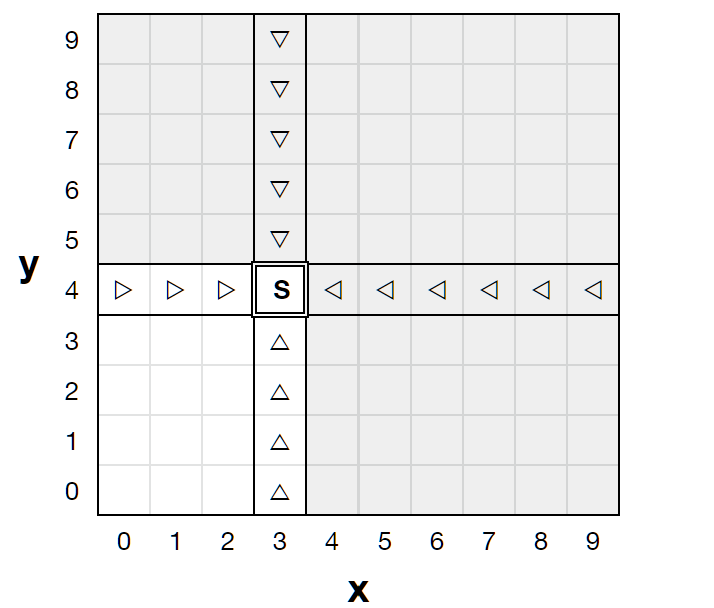
\includegraphics[width=0.4\textwidth]{a1q4new.png}
	      \end{center}
	      	              
	      \begin{enumerate} 
	      	\item (3 marks) The UQ water well company have decided to hire you - an algorithms expert - to devise a algorithm 
	      	      to find the water source as efficiently as possible. \\
	      	      	      	              
	      	      Describe (you may do this in words, but with sufficient detail) an algorithm to solve the problem of finding the water source, 
	      	      assuming you can break as many drill bits as you want. Provide a Big-O bound on the number of holes you need to drill to find 
	      	      it with your algorithm. Your algorithm should be as efficient as possible for full marks.\\\\
	      	      You may consult the hydrologists after any drill (and with a constant time complexity cost to do so) to see if 
	      	      the source is in the drilled row or column, and if so which direction the water source is in.\\\\
	      	      (Hint: A linear time algorithm is not efficient enough for full marks.)
	      	      
			\begin{Solution}

				It is possible to use a divide and conquer approach with two parts to identify the water source.
				\\
				\\
				To start off with, it is assumed that the action drilling runs in constant time and is able to identify if the drill bit is broken after it occurs. Furthermore, it is assumed that a drill is required before the hydrologists can be asked which direction the water source is in and if it is inline at all.
				\\
				\\
				The first part of the algorithm is called as a helper function and essentially acts as a binary search of the spaces in row 0 (y = 0) to identify the column that the water source is in. It will run as a single helper function that starts by drilling the centre of the given upper and lower bound and recursively calls itself with parameters dependent on if the drill bit was broken by the drilling. That is, the helper is first called with the input parameters $(m, n) = (0, n)$ representing the lower bound and upper bound of the search range. It starts by drilling at $((m + n)/2, 0)$, the centre of the search range, and consulting the hydrologists. If the hydrologists say that the water source is up from the current drilling location, that is the space drilled is in the same column as the water source, then the helper returns the column/y-value. Otherwise, if the drill bit breaks it calls itself with parameters $((m + n)/2, n)$ and if the drill bit is not broken after the drilling then it calls itself with parameters $(m, (m + n)/2)$. This way the algorithm recursively binary searches row 0.
				\\
				\\
				The second part of the algorithm is very similar to the first part but instead it binary searches column 0 to try and find the row the water source is in. This part does not require any information from the first part as it performs a second independent binary search. Similar to the first part the algorithm takes two parameters $m$ and $n$, which represent the lower and upper bound on column 0. The helper is first called with $(m, n) = (0, n)$ and it starts by drilling at $(0, (m + n)/2)$. After this the hydrologists are consulted and if the drilled location is inline with the water source then the current row of the drilled location is returned as the row/x-value of the water source. Otherwise, if the current location is not inline with the water source and the drill bit breaks then the helper recursively calls itself with parameters $(m, (m + n)/2)$. If the drill bit does not break then the helper calls itself with parameters $((m + n)/2, n)$. This way the search space is halved after each call and the search is much faster than linear time as explained further below.
				\\
				\\
				After both of these helper functions are called the algorithm has identified both the row and the column that the water source is in and thus the location of the water source. Those two values are returned.
				\\
				\\
				This algorithm drills $log(n)$ holes for the first helper and $log(n)$ holes for the second helper where $n$ is the height and width as defined in the question. This is because both sub-algorithms halve the potential search space on each of their recursive calls. Hence, the overall number of holes drilled can be said to be $2log(n) + a$ where $n$ is as defined in the question and $a$ is a constant representing any primitive operations called as initialisation and between the two helpers. As such, it can be said that this algorithm is $O(log(n))$.
	      	\end{Solution}
	      	      	      	              
	      	\item 
	      	      (5 marks) The company, impressed with the drilling efficiency of your algorithm, assigns you to another $n \times n$ grid, 
	      	      which also has a water source you need to help find. However, due to budget cuts, this time you can only break $2$ drill 
	      	      bits (at most) before finding the source. (Note that you are able to use a $3$rd drill bit, but are not allowed to ever break it).
	      	      	      	              
	      	      Write \textbf{pseudocode} for an algorithm to find the source while breaking at most $2$ drill bits, and give a tight Big-O 
	      	      bound on the number of squares drilled (in the worst case). If you use external function calls (e.g. to consult the hydrologist, 
	      	      or to see if the cell you drilled is the source) you should define these, their parameters, and their return values. \\\\
	      	      Your algorithm's time complexity should be as efficient as possible in order to receive marks. 
	      	      (Hint: A linear time algorithm is not efficient enough for full marks.)
	      	      
			\begin{Solution}
				\begin{algorithm}
					\begin{algorithmic}
						\Procedure{AskHydrologist}{int x, int y}
							\State $\textbf{return}$ Returns whether the water source is up, down, left or right of the location (x, y) using integers 1, 2, 3 and 4, respectively. If the location (x, y) is not inline with the water source and not the water source itself then 0 is returned. If the location (x, y) is a water source then 5 is returned.
						\EndProcedure
					\end{algorithmic}
				\end{algorithm}
				\begin{algorithm}
					\begin{algorithmic}
						\Procedure{Drill}{int x, int y}
							\State $\textbf{return}$ The location (x, y) is drilled and if the drill bit is unbroken 0 is returned, otherwise 1 is returned.
						\EndProcedure
					\end{algorithmic}
				\end{algorithm}
				\begin{algorithm}
					\begin{algorithmic}
						\Procedure{FindWaterSourceX}{int n, int startJumpSize}
							\State jumpSize $\gets$ startJumpSize
							\State currentX $\gets 0$
							\State previousX $\gets 0$
							\State drillResult $\gets$ Drill(currentX, 0)
							\\
							\While{drillResult != 1}
								\State previousX $\gets$ currentX
								\State currentX $\gets$ currentX + jumpSize
								\State jumpSize $\gets$ jumpSize - 1
								\State drillResult $\gets$ Drill(currentX, 0)
							\EndWhile
							\\
							\State currentX $\gets$ previousX
							\State Drill(currentX, 0)
							\State hydrologistResult $\gets$  AskHydrologist(currentX, 0)
							\While{hydrologistResult == 0}
								\State currentX $\gets$ currentX + 1
								\State Drill(currentX, 0)
								\State hydrologistResult $\gets$ AskHydrologist(currentX, 0)
							\EndWhile
							\\
							\State sourceX $\gets$ currentX
							\State $\textbf{return}$ sourceX
						\EndProcedure
					\end{algorithmic}
				\end{algorithm}
				\begin{algorithm}
					\begin{algorithmic}
						\Procedure{FindWaterSourceY}{int n, int startJumpSize}
							\State jumpSize $\gets$ startJumpSize
							\State currentY $\gets 0$
							\State previousY $\gets 0$
							\State drillReslt $\gets$ Drill(0, currentY)
							\\
							\While{drillResult != 1}
								\State previousY $\gets$ currentY
								\State currentY $\gets$ currentY + jumpSize
								\State jumpSize $\gets$ jumpSize - 1
								\State drillResult $\gets$ Drill(0, currentY)
							\EndWhile
							\\
							\State currentY $\gets$ previousY
							\State Drill(0, currentY)
							\State hydrologistResult $\gets$  
							\While{hydrologistResult == 0}
								\State currentY $\gets$ currentY + 1
								\State Drill(0, currentY)
								\State hydrologistResult $\gets$ AskHydrologist(0, currentY)
							\EndWhile
							\\
							\State sourceY $\gets$ currentY		
							\State $\textbf{return}$ sourceY
						\EndProcedure
					\end{algorithmic}
				\end{algorithm}
				\medskip
				\begin{algorithm}
					\begin{algorithmic}
						\Procedure{FindWaterSource}{int n}
							\State jumpSize $\gets ceil(0.5 * (sqrt(8 * n + 1) - 1))$
							\State sourceX $\gets$ FindWaterSourceX(n, jumpSize)
							\State sourceY $\gets$ FindWaterSourceY(n, jumpSize)
							\State $\textbf{return}$ (sourceX, sourceY)
						\EndProcedure
					\end{algorithmic}
				\end{algorithm}
				\medskip\newpage
				This algorithm works using a similar method to the previous algorithm, however instead of using binary search the size of the jump made is dynamic depending on how far the previous element was from the start of a row or column. 

				The first jump made for both searching the rows and columns is $k$ spaces long and each subsequent jump is $k - 1$, $k - 2$, $k - 3$, ... $1$ spaces long or a sequence where the sum of all terms is $\geq n$ where $n$ is the width and height of the grid. That isthe sum, $k + (k - 1) + (k - 2) + ... + 1 \geq n$ which is simplified to $\frac{k(k + 1)}{2} \geq n$. The solution of the above inequality is $k = \frac{1}{2}(\sqrt{8n + 1} - 1)$ and so the first jump's size must be $\left\lceil{(\frac{1}{2}(\sqrt{8n + 1}- 1))}\right\rceil$.

				The algorithm begins by searching columns using the above jump size as a starting point. When a drill is broken, it goes to the previous position and reduces its jump size to 1. This finds the column which the water source is in.

				A similar method is then employed to find the row the water source is in and the location of the water source is returned.

				As mentioned above the first jump is of size $\left\lceil{(\frac{1}{2}(\sqrt{8n + 1}- 1))}\right\rceil$, with each subsequent jump being one space smaller than the last. As the jump size decreases, the number of jumps required to search the space between jumps increases proportionally. That is, the size of the $i-th$ jump can be given by the formula $k - i$, where $k$ is the initial jump size and $i$ is the number of jumps made. Thus, since $i$ jumps are always required to reach a jump size of $k - i$ spaces, the most number of drills required is $k - i + i = k$, while the smallest is $k - i + 1$. Since $k$ is $\frac{n}{\frac{1}{2}(\sqrt{8n + 1}- 1))} = \frac{1}{4}(\sqrt{8n + 1} + 1) = \sqrt{\frac{1}{2}n + \frac{1}{16}} + \frac{1}{4}$ that is the maximum amount of drills required for a single side in the worst case. As such, for both sides the combined worst case is $\sqrt{2n + \frac{1}{4}} + \frac{1}{2}$ drills. Thus, this is a $O(\sqrt{n})$ algorithm.
			  \end{Solution}
	      \end{enumerate}     	          
\end{enumerate}
\end{document}